\documentclass{article}

% Formatting
\usepackage[utf8]{inputenc}
\usepackage[margin=1in]{geometry}
\usepackage[titletoc,title]{appendix}

% Math
\usepackage{amsmath,amsfonts,amssymb,mathtools}

% Algorithms
\usepackage[ruled,vlined]{algorithm2e}
\usepackage{algorithmic}
\usepackage{listings}

% Code syntax highlighting
\usepackage{minted}
\usemintedstyle{borland}

% Tree & Forest
\usepackage[edges]{forest}

\title{Homework 4}
\author{David Trinh}
\date{October 7, 2024}

\begin{document}

\maketitle

\begin{itemize}

    \item\textbf{ Question 1}

    \begin{enumerate}
        \item $b*ab*ab*$

        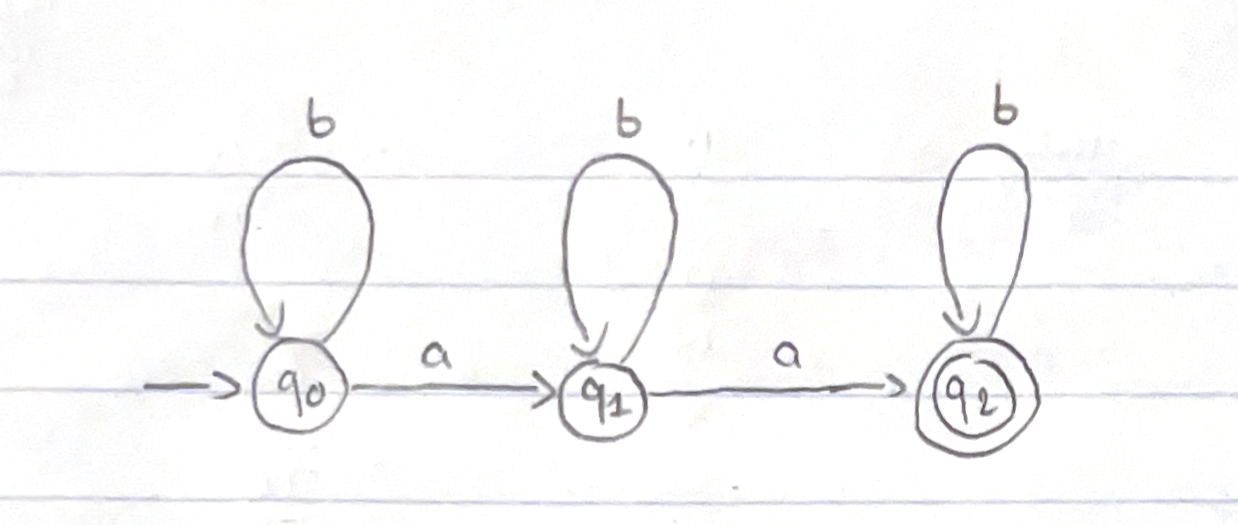
\includegraphics[scale=0.2]{HW4_Q1_1.png}

        \item $(ab|cd)*$

        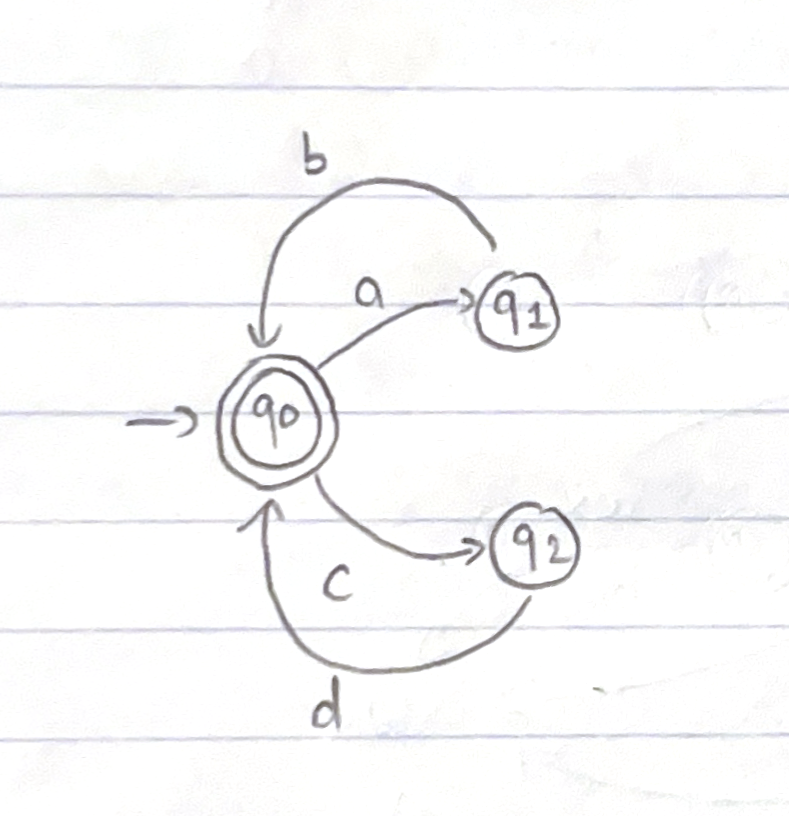
\includegraphics[scale=0.2]{HW4_Q1_2.png}

        \item $(a*ba*ba*)*$

        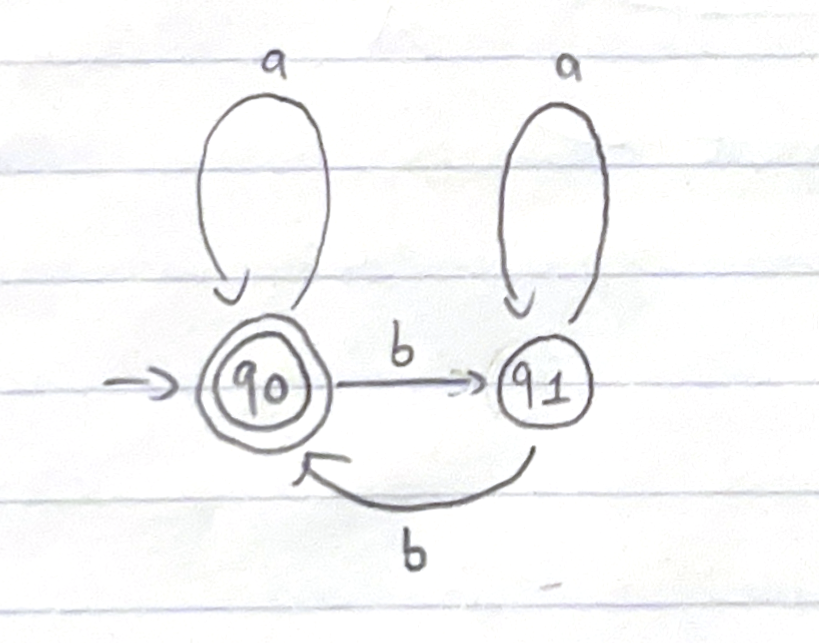
\includegraphics[scale=0.2]{HW4_Q1_3.png}
    \end{enumerate}

    \item\textbf{ Question 2}

    \begin{itemize}
        \item[] start state: $q_0$

        \item[] end state: $q_0, q_5$

        \item[] accept:     abb, bbaaab

        \item[] rejected:   aba, bbabab
    \end{itemize}
    


    \item\textbf{ Question 3}

        $(aab|bba)*$

    \item\textbf{ Question 4}

        \begin{itemize}
            \item \verb|\b|: Search for standalone strings (not joined to a word)
            
            \item \verb|(?:\d{1,2})[-/](?:\d{1,2})[-/](?:\d{2,4})|:
            
            This matches the formats \texttt{MM/DD/YY}, \texttt{MM/DD/YYYY}, \texttt{M/D/YYYY}, etc.
            
            \begin{itemize}
                \item \verb|\d{1,2}| matches a 1- or 2-digit month and day.
                \item \verb|[-/]| matches either a dash (\verb|-|) or a slash (\verb|/|) as separators.
                \item \verb|\d{2,4}| matches either a 2-digit or 4-digit year.
            \end{itemize}
            
            \item \verb|(?:\d{4})[-/](?:\d{1,2})[-/](?:\d{1,2})|:
            
            This matches the formats \texttt{YYYY/MM/DD}, \texttt{YYYY/M/D}, etc.
            
            \begin{itemize}
                \item \verb|\d{4}| ensures we are looking for a 4-digit year at the beginning.
            \end{itemize}
            
            \item \verb|(?:[A-Z][a-z]+) (?:\d{1,2}), (?:\d{4})|:
            
            This matches dates like \texttt{May 14, 2020}.
            
            \begin{itemize}
                \item \verb|[A-Z][a-z]+| matches the month, which starts with an uppercase letter and is followed by lowercase letters.
                \item \verb|\d{1,2}| matches a 1- or 2-digit day.
                \item \verb|, (?:\d{4})| matches a comma followed by a 4-digit year.
            \end{itemize}
            
            \item \verb|(?:\d{1,2}) (?:[A-Z][a-z]+), (?:\d{4})|:
            
            This matches dates like \texttt{14 May, 2020}. Similar to above just swapped the month and day around

            \item All terms above are in an OR statement.
            
        \end{itemize}


\end{itemize}

\end{document}